\section{Advective Entry: Role of Soil and Foundation}

The modeling in Chapter \ref{chp:preferential_pathways} help to explain why building pressurization influenced indoor air contaminant concentrations much more before the closing off of the sub-slab preferential pathway than after the closure.
The existence of the preferential pathway allowed advective transport to be the dominant transport mechanism for entry of contaminant vapors through the foundation breach.
This finding has wider implications for our understanding of the entry mechanics of VI.\par

It is commonly assumed that advective transport dominates in the near-foundation region and through breaches in the foundation itself, but our modeling of the situation at the ASU house showed that this was mainly possible because:
\begin{enumerate}
  \item The preferential pathway represented a source from where air could readily be drawn drawn into the subslab region.
  \item The permeable gravel sub-base acted as a communication medium between the preferential air source and the building.
\end{enumerate}
In other words, for advective transport to dominate through foundation cracks, some site-specific features were required.
We showed that absent the preferential pathway, the soil surrounding the house itself presented too much resistance to air flow for this to be possible.\par

Only one soil type was explored in the modeling work in Chapter \ref{chp:preferential_pathways} - sandy clay.
This kind of soil is a relatively impermeable soil, and other soil type are now considered.
Furthermore, our modeled house featured a basement, and in such a scenario, the atmosphere is relatively far removed from the foundation breach, and thus it makes sense to also consider a slab-on-grade type of foundation.\par

\begin{figure}[htb!]
  \centering
  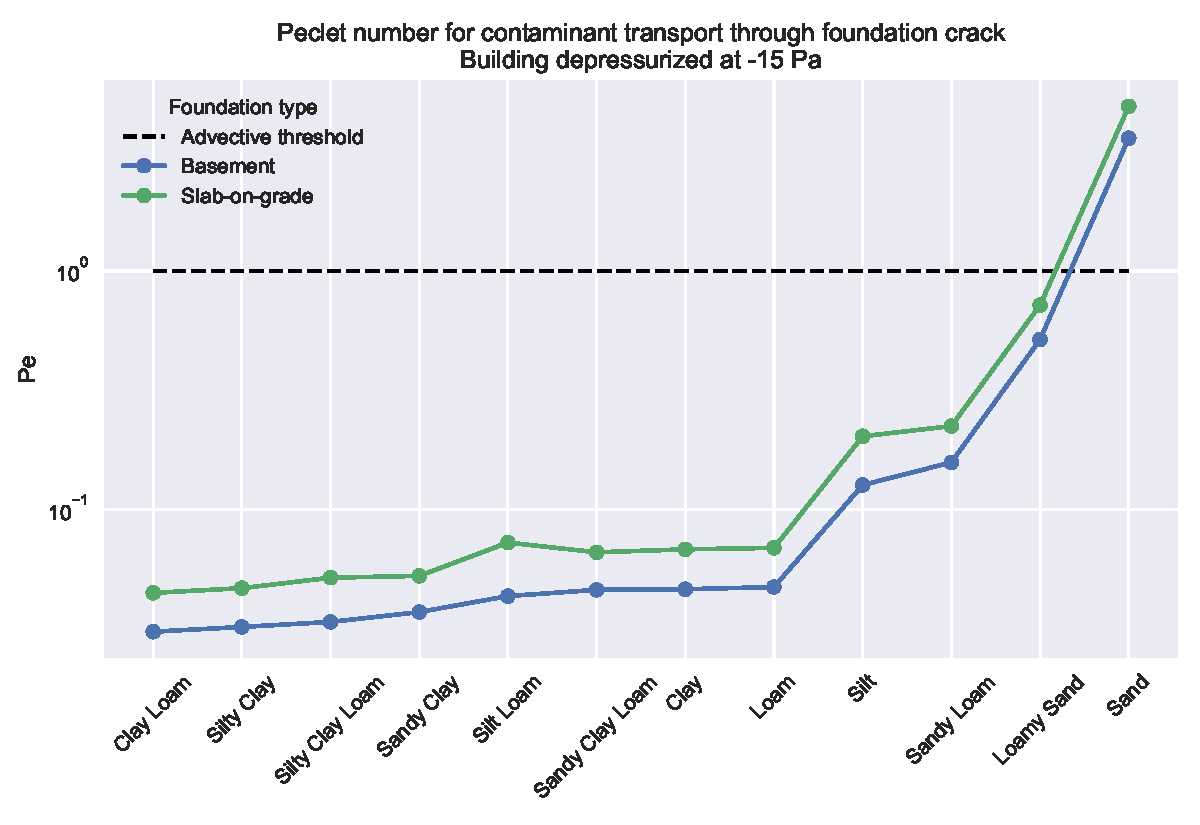
\includegraphics[width=\textwidth]{peclet_cases.pdf}
  \caption[Predicted effect of soil and foundation type on the Péclet number of transport through the foundation crack.]{Predicted effect of soil and foundation type on the Péclet number of transport through the foundation crack. We consider the 12 different soils studied by the EPA (see Table), and for each of these we consider a house featuring a basement and a slab-on-grade house. The foundation slab is assumed to be \SI{15}{\centi\metre} thick. In the basement case, the bottom of the foundation slab is assumed to be \SI{1}{\metre} bgs and in the slab-on-grade case  \SI{15}{\centi\metre} bgs. The modeled building is assumed to be depressurized at \SI{-15}{\pascal}. The threshold where advective contaminant entry begins to overtake diffusive entry, i.e $\mathrm{Pe} = 1$, is marked by the dashed line.}
  \label{fig:peclet_soil_foundation_type}
\end{figure}

The effect of different soil and foundation types is investigated using the model already introduced in Chapter \ref{chp:modeling}.
We consider 12 of the soil types defined by the EPA (see Table \ref{tbl:soils}) and for each of these we consider a basement and a slab-on-grade case respectively.
The basement and slab-on-grade cases are defined by the bottom of a foundation slab located at \SI{1}{\metre} and \SI{15}{\centi\metre} bgs respectively.
The building is assumed to be depressurized at $p_{in} = \SI{-15}{\pascal}$, a value somewhat greater than "normal", in order to enhance the advective entry potential.
The analysis in Chapter \ref{chp:preferential_pathways} already showed that for the case of existence of a gravel sub-base layer, absent an air source supplied by a preferential pathway, results were was virtually indistinguishable from the cases where there was no gravel sub-base layer.
I.e. a gravel sub-base will not be included in the model.\par

The results of the calculations will be shown in terms of the Péclet number for the modeled contaminant entry pathway.
This Péclet number is defined as already shown before in equation \eqref{eq:peclet_number} as:
\begin{equation}
    \mathrm{Pe} = \frac{\mathrm{advection}}{\mathrm{diffusion}} = \frac{u_\mathrm{ck} L_\mathrm{slab}}{D_\mathrm{g}}
\end{equation}
here $u_\mathrm{ck}$ [\si{\metre\per\second}] is the airflow velocity across (through) the crack
$L_\mathrm{slab} = \SI{15}{\centi\metre}$ is the thickness of the foundation slab, i.e. the characteristic length for transport;
and $D_g = \SI{6.87e-6}{\metre\squared\per\second}$ is the diffusivity of TCE in air.\par

\begin{figure}[htb!]
  \centering
  \begin{subfigure}{0.75\textwidth}
    \centering
    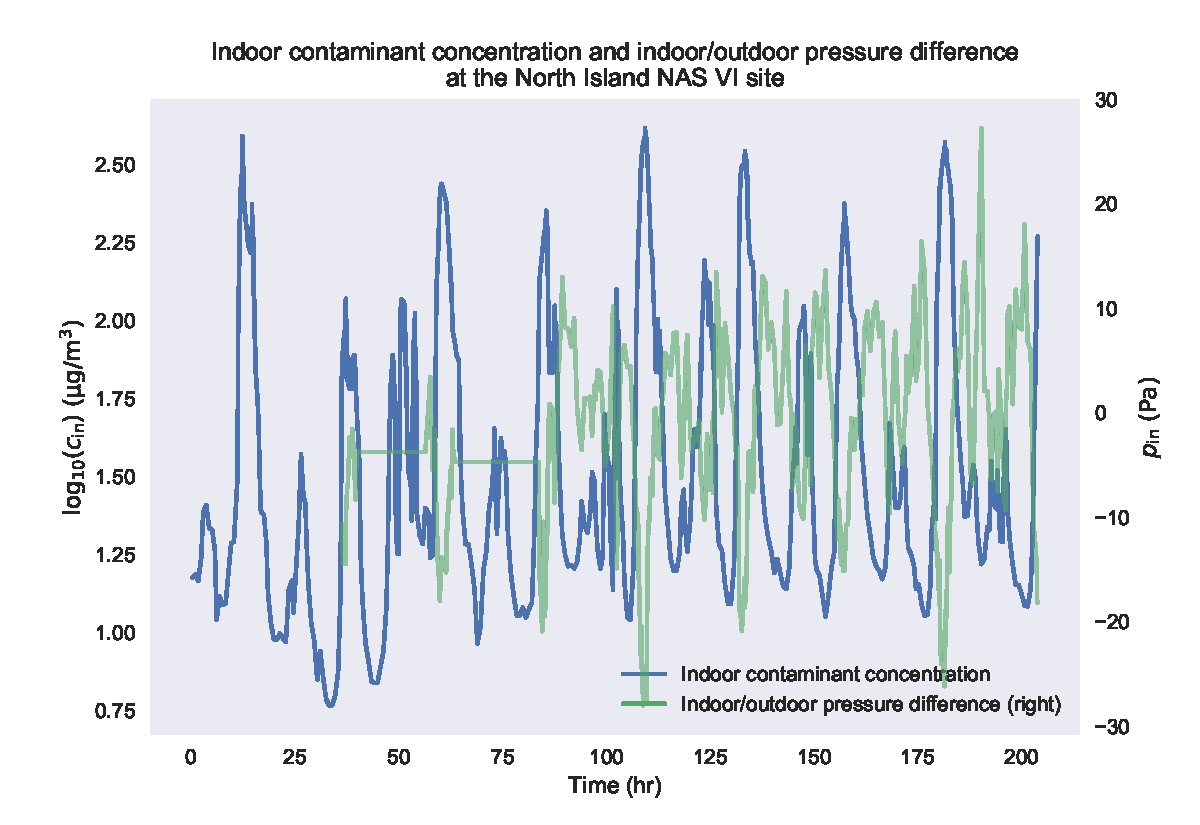
\includegraphics[width=\textwidth]{nas_indoor_conncentration_pressure.pdf}
    \caption[Time series of the indoor contaminant concentration and indoor/outdoor pressure difference at the North Island NAS VI site.]{Time series of the indoor contaminant concentration and indoor/outdoor pressure difference at the North Island NAS VI site. A negative pressurization value here indicate that there is a net flow of air into the building.}
  \end{subfigure}
  \begin{subfigure}{0.75\textwidth}
    \centering
    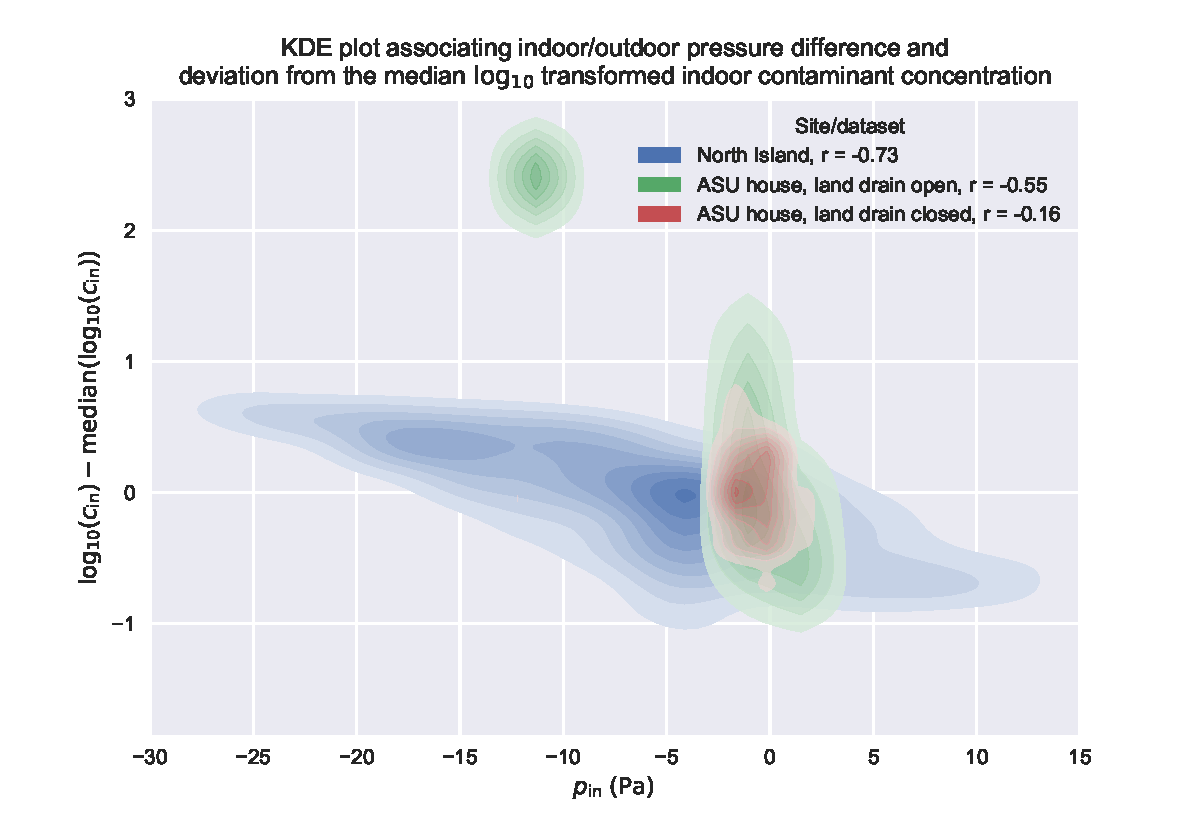
\includegraphics[width=\textwidth]{indoor_pressure_kde.pdf}
    \caption[KDE plot comparing indoor contaminant concentration and indoor/outdoor pressure difference at North Island NAS and the ASU house.]{Kernel density estimation (KDE) plot of indoor contaminant concentration $c_\mathrm{in}$ and indoor/outdoor pressure difference $p_\mathrm{in}$ at North Island NAS and the ASU house (considering the periods when the land drain was open and closed respectively). Indoor contaminant concentrations are $\log_{10}$ transformed and normalized to their respective median values to allow comparison of how building pressurization contributed to indoor contaminant concentration variability. A deeper color indicates that the two variables are more closely associated. Pearson's r values of $\log_{10}(c_\mathrm{in})$ and $p_\mathrm{in}$ for each dataset were also calculated.}
  \end{subfigure}
  \caption{Building pressurization and indoor contaminant concentration were highly correlated at the North Island Naval Air Station (NAS) VI site.}
  \label{fig:north_island}
\end{figure}

The result of these model calculations are shown in Figure \ref{fig:peclet_soil_foundation_type}.
These results shows that for most soil types, irrespective of whether a building has a basement or a slab-on-grade foundation, the Péclet number across the foundation slab is actually not sufficiently high for advection to be the dominant entry mechanism; most soils are too impermeable for sufficient airflow to be pulled into the building by the small pressure gradient that exists between the building interior and the subsurface.
Sites characterized by sandy soil are an exception to this, as they are permeable enough to sustain such airflows.\par

An example of such a site is a site at North Island Naval Air Station (NAS) in San Diego, California, characterized by sandy soil.
There the indoor contaminant concentration and building pressurization were highly correlated\cite{hosangadi_high-frequency_2017}.
Figure \ref{fig:north_island} demonstrate this correlation by showing the fluctuating indoor contaminant concentration and building pressurization at North Island NAS over time.
Figure \ref{fig:north_island} also includes a kernel density estimation (KDE) plot of the building pressurization and indoor contaminant concentration.
The KDE plot and calculated Pearson's r values show that indoor contaminant concentration and building pressurization was even more strongly associated at North Island NAS than the ASU house when the preferential pathway was open.
This strong correlation can partly be attributed to the sandy soil at the site, but also to the significant building pressurization fluctuations at the site (compared to the ASU house).\par

In contrast, \citeauthor{hers_evaluation_2014}\cite{hers_evaluation_2014} studied a VI site in North Battleford, Saskatchewan, Canada, where they continuously monitored oxygen, pressure differentials, soil temperature, soil moisture, and weather conditions.
The recorded data was used together with a reactive transport model (MIN3P-DUSTY) to simulate biodegradation and transport at the site.
Together with analysis of the site data, they concluded that contaminant transport was dominated by diffusion, and little association between building pressurization and contaminant entry existed.\par

This indicates that for many sites characterized by other soil types, significant advective transport of contaminant vapors into the building is likely to be possible in the presence of some preferential air source.
It is important to note however, that preferential pathways can be of many types, not just the one case that we have considered in Chapter \ref{chp:preferential_pathways}.
For example, having a layer of loose, unconsolidated soil adjacent foundation walls might in some cases provide a low resistance pathway to flow of air to the subslab region.\par

The consequences of this analysis are important when considering the application or interpretation of certain types of vapor intrusion investigation strategies.\par
\clearpage
\newpage
